\chapter{The ATLAS Detector}\label{ch:atlas}

ATLAS is a system of particle detectors built to measure collisions of both proton-proton and heavy ion collisions
generated by the LHC.\cite{atlas-detector-2008}
The full detector is $44~m$ long and $25~m$ in diameter.
It consists of an inner detector subsystem for charged particle tracking and electron identification,
electromagnetic and hadronic calorimeters, and a muon spectrometer.

\section{Coordinates}\label{sec:coordinates}
The coordinate system used in this document is the standard ATLAS coordinate system, detailed here.
For both Cartesian and polar coordinates, the origin is defined as the nominal interaction point.
The z-axis points down the beamline.
The x-y plane is perpendicular to the beamline.
The positive y-direction points up, and the positive x-direction points towards the center of the LHC ring.
The positive z-direction therefore points counterclockwise along the LHC, when viewed from above,
as required by a right-handed coordinate system.

For cylindrical coordinates, the z-axis is defined the same way as for
Cartesian coordinates. The azimuthal angle $\phi$ is the angle
from the positive x-axis, while the polar angle $\theta$ is the angle
from the beamline.

A more convenient measure of angle from the beamline is the
\textit{rapidity}, because rapidity differences are invariant under Lorentz boosts in the
z-direction.
Rapidity is defined as:
\begin{equation}
y = \frac{1}{2}\ln\frac{E+p_z}{E-p_z}
\end{equation}

Another frequently used quantity is the
\textit{pseudorapidity}, which is defined as:
\begin{equation}
\eta = -\ln\frac{\theta}{2}
\end{equation}

Pseudorapidity differences are also invariant with respect to
longitudinal Lorentz boosts. In the limit where $p_T \ll m$, rapidity and
pseudorapidity are equal.

Pseudorapidity ranges from zero to plus or minus infinity.
The x-y plane, which is perpendicular to the beamline, is described by a pseudorapidity $\eta=0$.
The z-axis, which is parallel to the beamline, is described by pseudorapidity $\eta=\pm\infty$

Finally, a distance measure in $\eta-\phi$ space is often used, especially when describing jets.
This distance, $\Delta R$ is defined as:

\begin{equation}
\Delta R = \sqrt{\Delta\eta^2+\Delta\phi^2}
\end{equation}

\section{Magnet Systems}\label{sec:magnet_systems}
The two ATLAS magnet systems are used to curve the tracks of charged particles passing through the detector,
so that their momenta can be measured.

The layout of the magnet systems can be seen in figure~\ref{fig:magnet_layout}.

\begin{figure}[h]
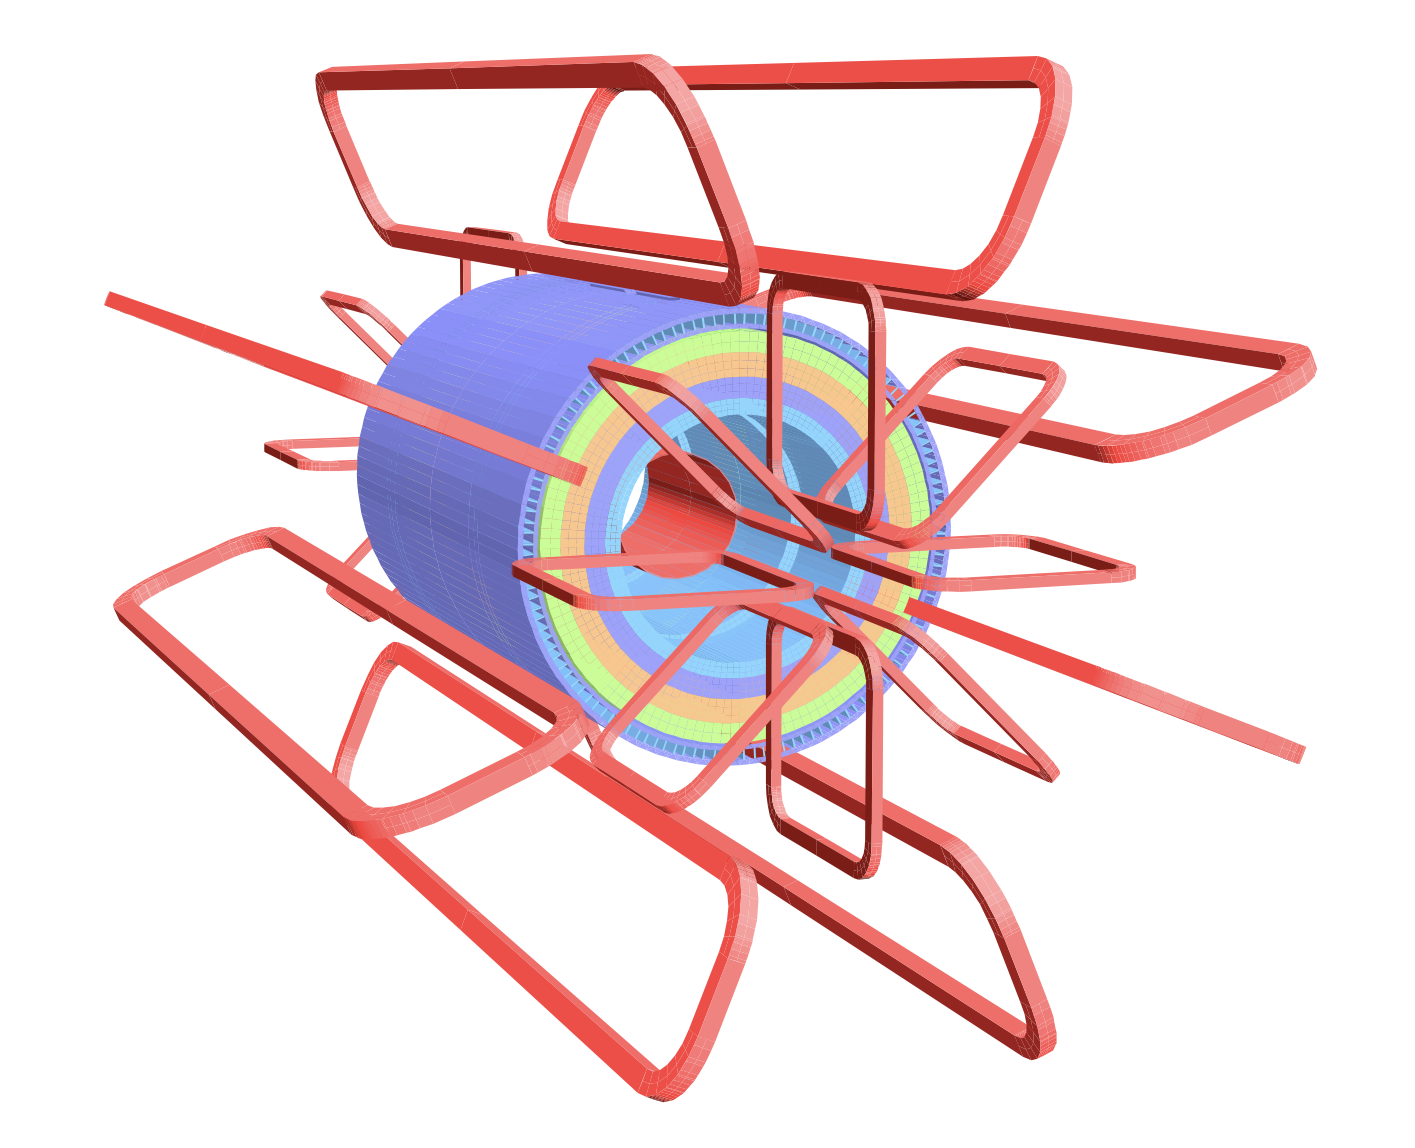
\includegraphics[width=\textwidth]{magnet_layout}
\caption{A diagram showing the layout of the ATLAS magnet system.
The central solenoid is used to apply a force that curves the trajectories of charged particles in the inner detector.
In red are the toroid coils, used to bend the tracks of charged particles passing through the muon spectrometer.}
\label{fig:magnet_layout}
\end{figure}

The first magnetic field is produced by the central solenoid, which surrounds the entire inner detector,
and is surrounded by the barrel calorimeters.
It generates a uniform $2~T$ axial magnetic field in the inner detector.
The coils are made of Al-stabilized NbTi. The length is $5.8~m$, and the outer diameter is $2.56~m$\cite{atlas-detector-2008}.

The second magnet system, used to bend the trajectories of muons passing through the muon spectrometer,
has a more complicated geometry.
It consists of a barrel toroid section, and two symmetrical end-cap toroids.
The exact shape of the resulting magnetic field is quite complex,
but roughly runs in a circular direction around the calorimeters.

The axial length of the barrel toroid is $25.3~m$, and the outer diameter measures $20.1~m$.
The average field strength is $0.5~T$ and the superconducting material used is similar to that used in the
central solenoid\cite{atlas-detector-2008}.
Figure~\ref{fig:toroid_end_view} shows an end-on view of the barrel toroid, after installation,
and before the calorimeters are inserted.

\begin{figure}[h]
\includegraphics[width=\textwidth]{toroid_end_view}
\caption{A picture of the ATLAS barrel toroid after installation. In
  the center of the image is the calorimeter and central solenoid,
  before being moved into the final position.}
\label{fig:toroid_end_view}
\end{figure}

The end-cap toroids are used to generate the magnetic field for muons passing through the end-cap region of the muon spectrometer.
The properties and geometry of the end-cap toroids are similar to the barrel toroid,
with peak magnetic field reaching $4.1~T$\cite{atlas-detector-2008}.

\section{Inner Detector}\label{sec:inner_detector}
The inner detector consists of silicon pixel detectors, silicon strip detectors, and transition radiation trackers.
It covers a region from $R = 33~mm$ to $R = 1082~mm$ and $|\eta| = 0$ to $|\eta| = 2.5$.
The entire inner detector is immersed in a $2~T$ magnetic field, generated by a
solenoid coil which surrounds it.\cite{atlas-detector-2008}
The layout of inner detector subsystems is shown in figure~\ref{fig:inner_detector_quarter}.

\begin{figure}[h]
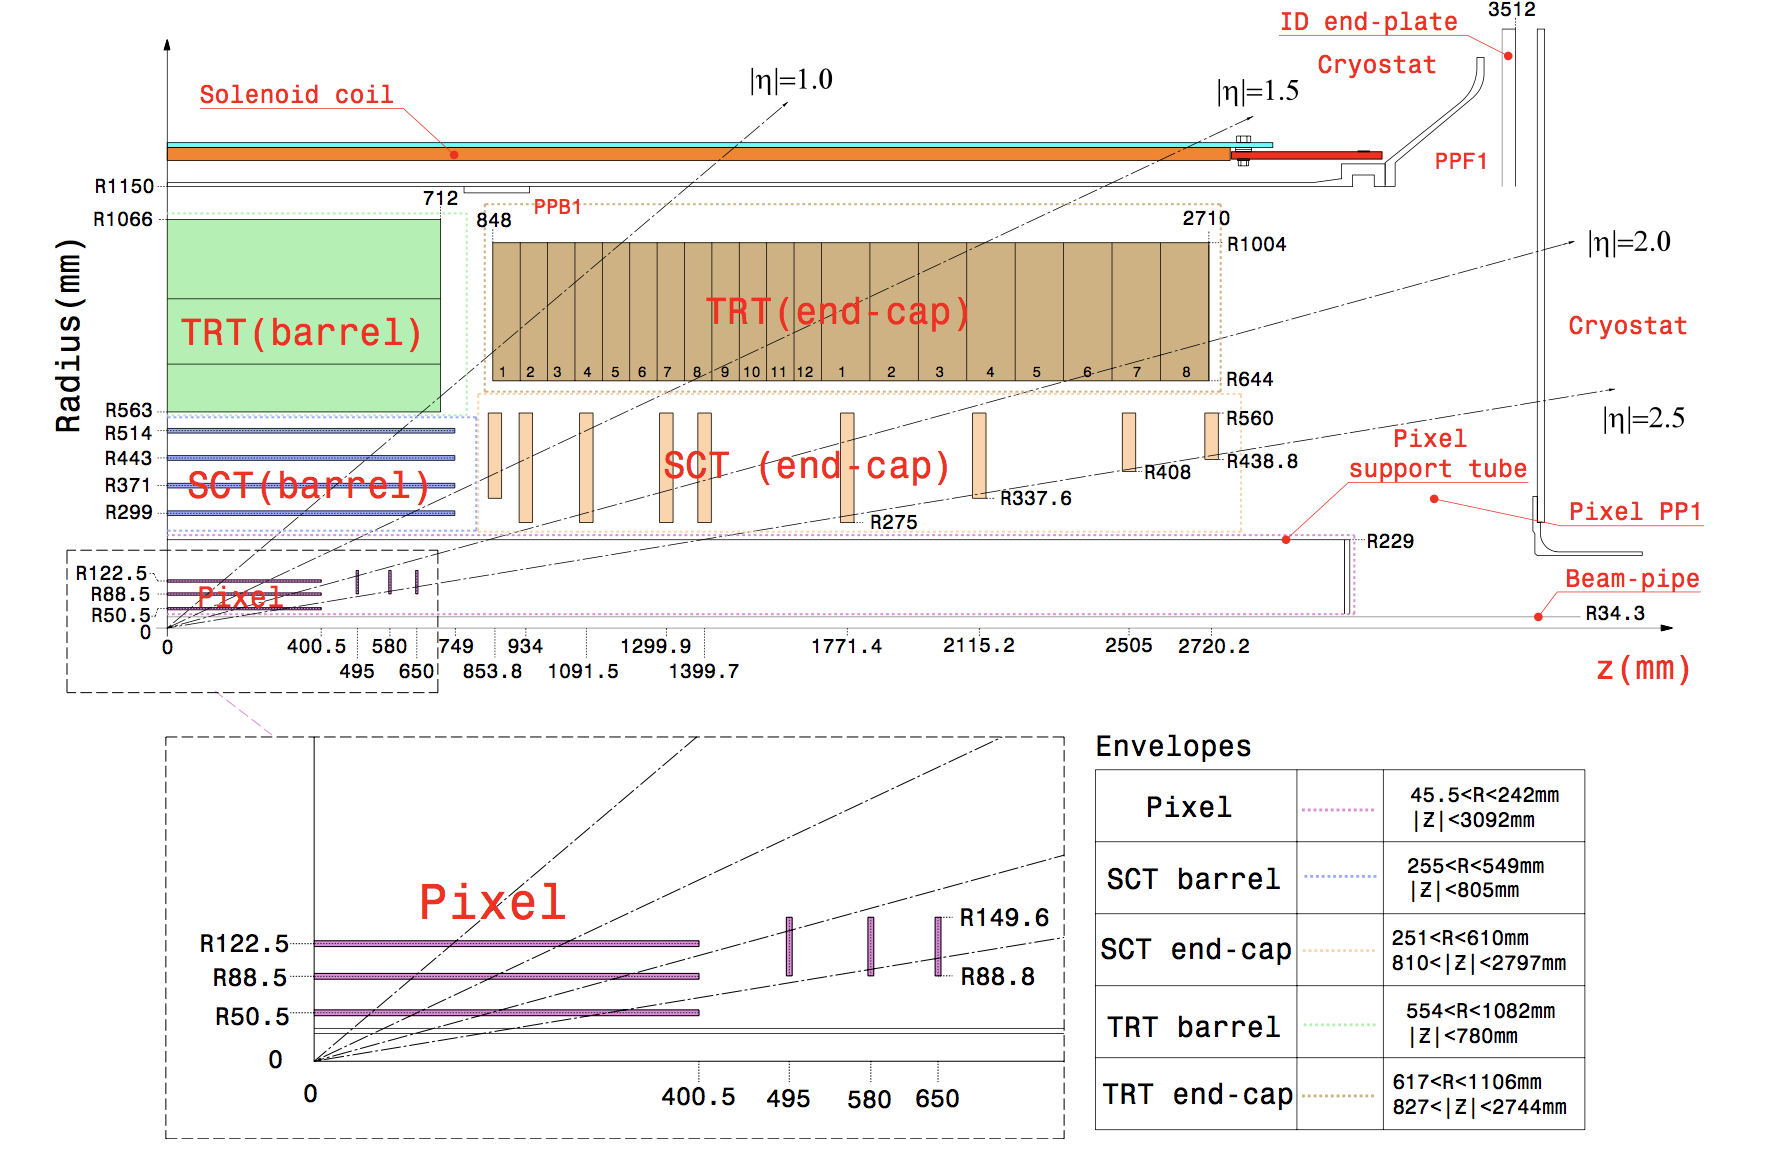
\includegraphics[width=\textwidth]{inner_detector_quarter}
\caption{A quarter-section plan showing the layout of inner detector susbystems and their dimensions.
Not shown is the innermost layer of the pixel detector, the IBL, which was installed in May 2014.}
\label{fig:inner_detector_quarter}
\end{figure}

\subsection{Pixel Detector}\label{subsec:pixel}

The innermost layer of ATLAS detectors is the pixel system.
Since it lies closest to the interaction point, the pixel system experiences the highest flux of any ATLAS subdetector.
This means that the pixel detector must have the greatest radiation hardness, greatest resolution,
and greatest occupancy of any subdetector.\cite{atlas-detector-2008}
The pixel system consists of 1744 solid-state pixel sensors, arranged into a barrel region and two endcap regions.
In total, there are 80.4 million pixel readout channels.\cite{atlas-detector-2008}

\subsubsection{Layout}
The barrel region consists of four concentric cylindrical layers, coaxial with the beamline.
The two endcap regions are each made up of three disks, arranged perpendicular to the beamline.

The pixel barrel envelope covers a region from $z = 0$ to $|z|  = 400.5~mm$.
The four layers are located at increasing distances from the beamline, at $R = 33~mm, 50.5~mm, 88.5~mm, 122.5~mm$.

The six endcap disks are located at $|z| = 495~mm, 580~mm, 650~mm$ and cover the region $88.8~mm < R < 149.6~mm$.\cite{atlas-detector-2008}

Figure~\ref{fig:inner_detector_quarter} shows a quarter-section of
the entire inner detector, as well as a detailed view of the pixel
subsystem, not including the Insertable B Layer (IBL), which was
installed in 2014.

\subsubsection{Sensors}
The ATLAS pixel sensors are solid-state silicon detectors.
The basic operating principle of a solid-state detector is that charged particles passing through the material
generate electron-hole pairs, which are accelerated towards opposite ends of the material via an electric field.
This generates a current, which can be measured by charge-sensitive sensors at the edge of the material.\cite{spieler-2005}

In a silicon detector, the active material is a pn junction, operated with a reverse bias voltage,
until fully depleted.
This reduces the thermal noise from free charge carriers to a low enough level that electron-hole pairs
from signal particles can be detected.\cite{spieler-2005}

In ATLAS, the pixel sensors consist of an n-type bulk, with $p^+$ implants on the back side and $n^+$ implants on the front side.
Before irradiation, the active pn junction region exists between the n-type bulk and $p^+$- implanted side.
Irradiation leads to the reduction in the effective doping concentration,
until the bulk material undergoes type inversion.
After type inversion, the active pn junction region switches to the $n^+$-doped side.\cite{pixels-2008}
This process is illustrated in figure~\ref{fig:pixel_type_inversion}.

This $n^+$-in-$n$ design allows the sensors to continue to operate both before and after large doses of radiation.

Each pixel tile has 47232 pixels, laid out in a grid of 144 columns by 328 rows.
Some of the pixels are grouped to common read-out channels, resulting in 46080 read-out channels.
This grouping is done so that an equal number of read-out channels can be connected to each of
the 16 front-end read-out chips.\cite{pixels-2008}

In 128 of the columns, each pixel implant is $382.5\times30~\mu m^2$, with pitch (center-to-center distance) of  $400\times50~\mu m^2$.
In the remaining 16 columns, the pixel sizes are $582.5\times30~\mu m^2$, with a pitch of  $600\times50~\mu m^2$.\cite{pixels-2008}

\begin{figure}[h]
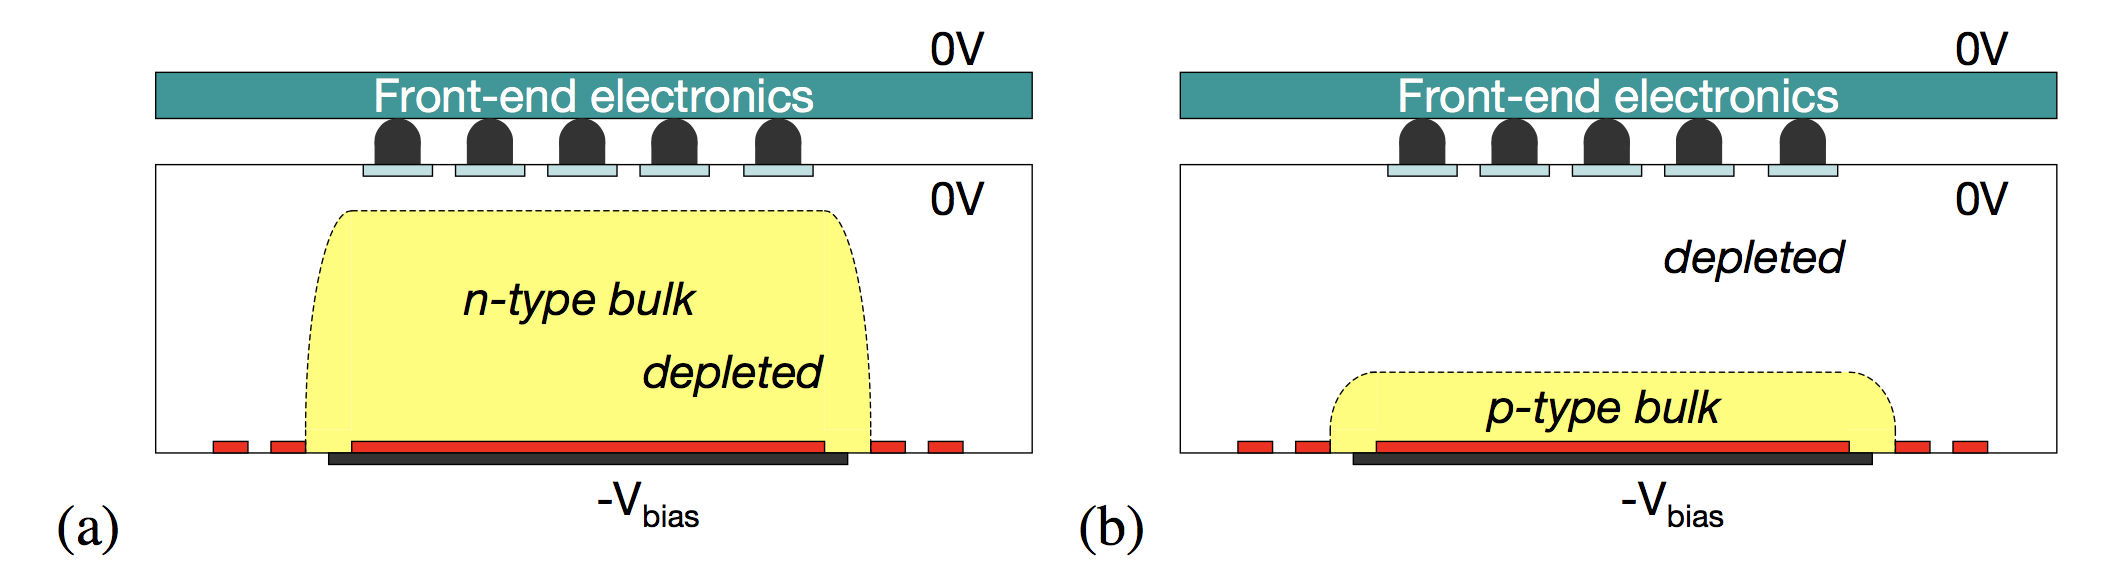
\includegraphics[width=\textwidth]{pixel_type_inversion}
\caption{Graphic illustrating how $n^+$-in-$n$ pixel sensors continue to operate after the type inversion that results from irradiation.
In (a), the unirradiated state, the bulk is n-type, and the depletion zone occurs between the $p^+$-doped back side.
After type inversion, in (b), the depletion zone occurs between the now p-type bulk and the $n^+$-doped front side.
\cite{pixels-2008}}
\label{fig:pixel_type_inversion}
\end{figure}

\subsubsection{The IBL}
A major upgrade that occurred during the long shutdown in 2014 was to install the Insertable B-Layer (IBL) to the pixel detector.
The IBL became the fourth and innermost layer of the pixel detector.
The IBL provides several key improvements to the tracking system, which will allow the pixel detector to maintain
good performance even in the higher-luminosity environment that will be present in the High Luminosity LHC (HL-LHC).\cite{ibl-tdr}
The IBL does this by improving tracking robustness against module failures,
adding measurement redundancy to mitigate the effects of pileup,
and adding an additional measurement closer to the interaction point.\cite{ibl-tdr}

As part of the IBL insertion project, the original beam pipe was removed, and replaced with a smaller-radius beampipe.
Precision tooling and methods for insertion were developed and practiced for two years before the procedure was finally carried out.
The tolerances were extremely tight, with only a $0.2~mm$ gap between the IBL and inner supporting tube.\cite{ibl-website}.
An image of the IBL being inserted can be seen in figure~\ref{fig:ibl_insertion}

\begin{figure}[h]
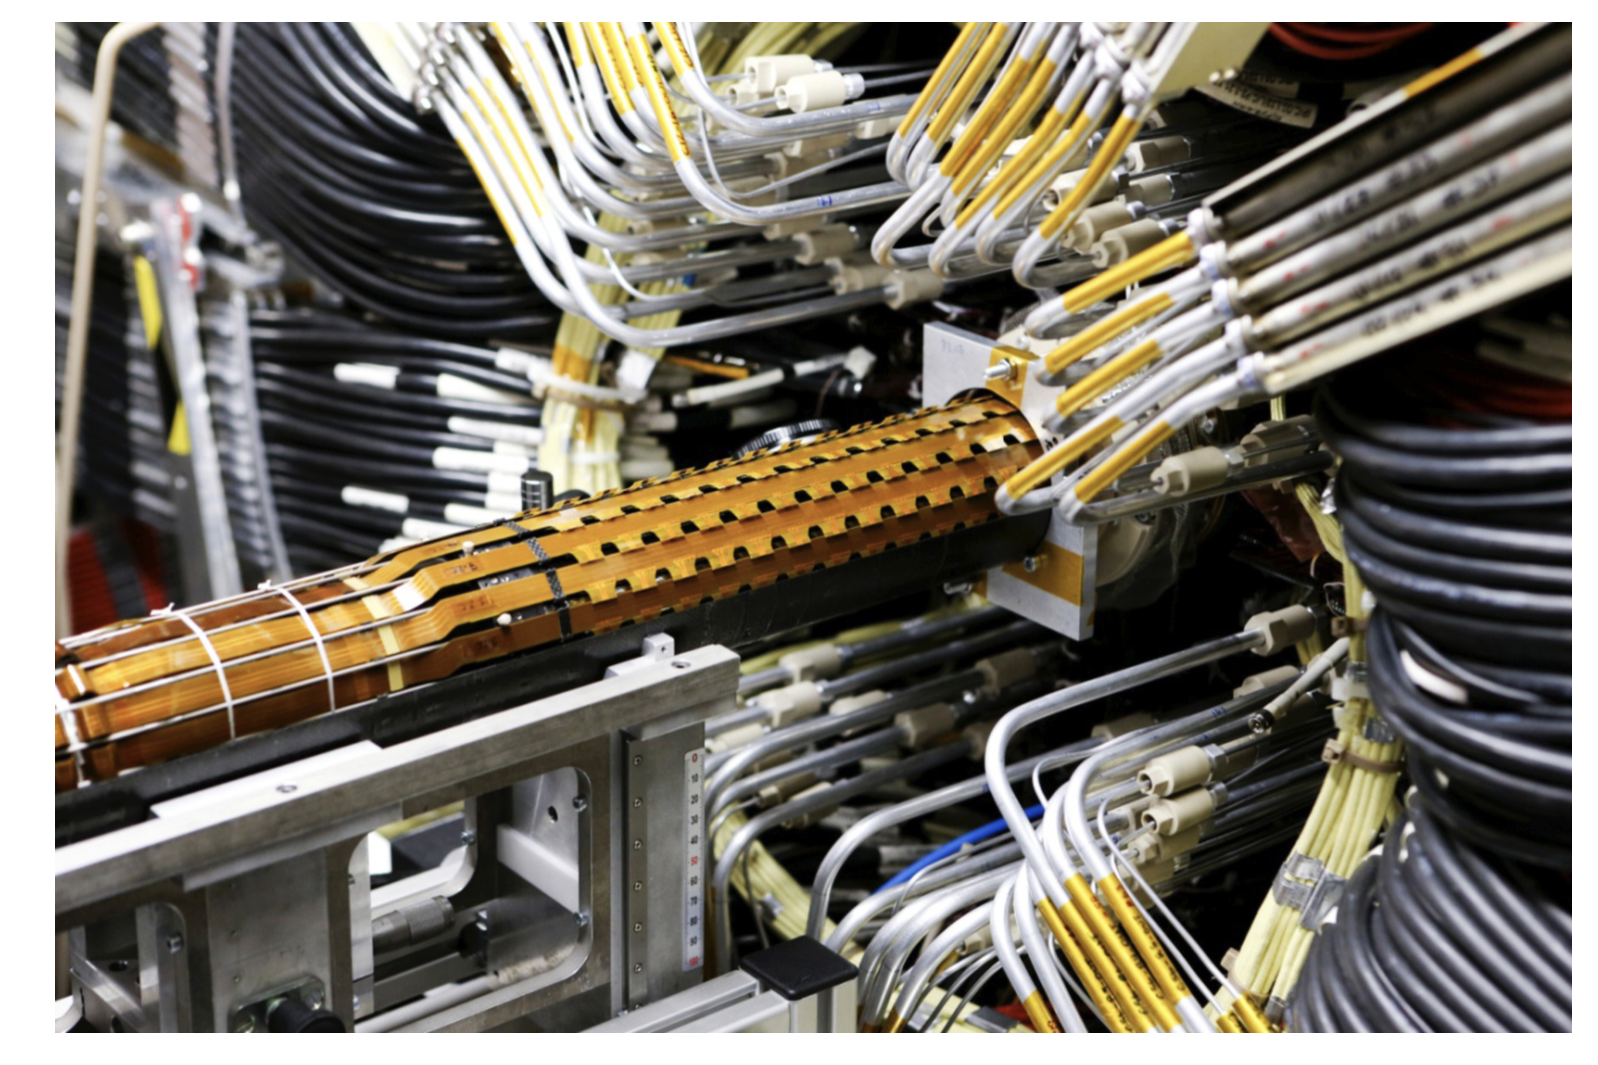
\includegraphics[width=\textwidth]{ibl_insertion}
\caption{The IBL as it was inserted into the pixel detector}
\label{fig:ibl_insertion}\cite{ibl-website}
\end{figure}

\subsection{Silcon Strip Tracker}\label{subsec:sct}

After the pixel detector system, the next innermost subdetector is the SemiConductor Tracker, or SCT .
The SCT consists of 4088 modules, with a total silicon surface area of $63~m^2$.\cite{atlas-detector-2008}
The SCT sensors are silicon strips rather than pixels.
In order to obtain two-dimensional resolution, SCT modules are paired back-to-back at a small stereo angle.

\subsubsection{Layout}
Like the pixel system, the SCT barrel region consists of four concentric cylindrical layers, coaxial with the beamline.
The two endcap regions are each made up of nine disks, arranged perpendicular to the beamline.

The SCT barrel envelope covers a region from $z = 0$ to $|z|  = 746~mm$,
and the four layers are located at increasing distances from the beamline,
at $R = 299~mm, 371~mm, 443~mm, 514~mm$.\cite{sct-barrel-2006}

The nine endcap disks on each side range from $|z| = ~mm$ to $|z| = ~mm$,
and cover the region $275~mm < R < 560~mm$.\cite{atlas-detector-2008}

The modules are arranged in back-to-back pairs at a stereo angle of $40~mrad$, in order to provide two-dimensional resolution.

\subsubsection{Modules}
Like in the pixel system, the SCT sensors are solid-state silicon detectors.
Instead of pixels, the base unit is a strip of silicon, ranging in length from $6$ to $13~cm$.
These strips are made of p-type silicon, and are embedded in n-type silicon. The average pitch is $80~\mu m$.\cite{sct-2008}

The resolution resulting from this design is $17~\mu m$ in the $r-\phi$ direction, and $580~\mu m$ in the z-direction.\cite{sct-2008}

\subsection{Transition Radiation Tracker}\label{subsec:trt}
Moving outwards from the pixel system and SCT, the final inner detector subsystem is the transition radiation tracker, or TRT .
Unlike the pixel or SCT systems, the TRT uses proportional drift tubes, referred to as straws, as sensors.

\subsubsection{Layout}
\subsubsection{Modules}

The TRT uses proportional drift tubes to detect charged particles.
A tube is filled with a mixture of two or more gases, including an inert gas such as Xenon, and an electric field is applied across the tube.
When a charged particle passes through the tube, ion pairs are generated from the inert gas.
Positive and negative ions drift in opposite directions, towards the cathode and anode, respectively.
If a particle's energy is completely absorbed in the tube, the number of ions produced in stopping the particle is
proportional to the original energy of the particle.\cite{knoll-2000}

In the ATLAS TRT, the straws are filled with a mixture of $70\%~\mathrm{Xe}$, $27\%~\mathrm{CO_2}$,
and $3\%~\mathrm{O_2}$.
Carbon dioxide is used as a quencher gas, which is needed to guarantee that the ionizaiton procedure is stable.
The addition of a small amount of oxygen increases the voltage difference between the working point and the breakdown voltage,
further stabilizing the process.\cite{trt-2013}


\section{Calorimeters}\label{sec:calorimeters}
\subsection{Electromagnetic Calorimeters}\label{subsec:em_cal}
\subsection{Hadronic Calorimeters}\label{subsec:had_cal}
\section{Muon Spectrometer}\label{sec:muon_spec}
\section{Trigger and Data Acquisition}\label{sec:trigger}